\section{Interaction Design}
A very important part when developing the application to fit a pleasurable user experience is to make sure that it works as flawless as possible, and there are no misinterpretations when using the product. For the artefact that is going to be developed, the “traditional” interaction methods do not cover the functionalities that are needed to cover our initial concept needs. To assure that the alternative interaction is integrated in a convenient manner, knowledge about different sensors and possible combination of two or more to make more intelligent outcomes should be established.
\subsection{Traditional interaction methods and their replacement}
As technology evolves, new ways of interacting with computational devices are constantly built. With that, people’s needs also change. The transition from the classical buttons on a cellphone to a touchscreen has made new ways of interaction possible - the delimitation of physical buttons made it available to have any customised graphical interfaces on the screen possible. This made life easier for casual tasks - like zooming a photo using two fingers as multi-touch input, which is much more intuitive than the classical button alternative.
The smartphone technology evolved further, where different sensors have started finding their place in smart devices. Soon enough there were devices with GPS, WiFi, Bluetooth, Light sensor, Camera, and other sensors. The implementation of these sensors in the smartphone allowed new forms of interaction, such as video calling, flashlight and screen orientation.
%\begin{itemize}
%\item mention immersion
%\item if sensors are used well - sharpness achieved. beneficial for imitating %feeling of reality
%\item conclusion (non-traditional)
%\item what sensors we are going to use and why
%\end{itemize}

\subsubsection*{The Accelerometer}
The accelerometer is capable of detecting the force and the movement in a three-dimensional space. This feature is most commonly used to adjust the display to match the position that the device is held in by the user (Chong, r.(year?) ). If the accelerometer is rotated at the center of the system, however, it will not detect the movement. Accelerometer, along with other sensors is commonly used in the augmented reality concepts (examples 1, 2).
\subsubsection*{The Gyroscope}
A gyroscope is a device that uses Earth's gravity to help determine orientation. Its design consists of a freely-rotating disk called a rotor, mounted onto a spinning axis in the center of a larger and more stable wheel. As the axis turns, the rotor remains stationary to indicate the central gravitational pull, and thus which way is "down."(Ryan Goodrich, 2013). Gyroscope, in comparison to magnetometer and accelerometer, is the physically largest and most expensive sensor, so the possible limitations in the smart devices in-built Gyroscopes have to be considered. 
%http://issuu.com/eeweb/docs/01-2015_embedded_developer_2_pages/30?e=7607911/11184384

\begin{figure}[H]
\centering
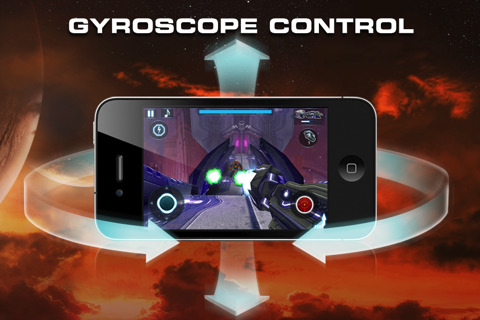
\includegraphics[scale=0.5]{GyroscopeApp.jpg}
\caption{iPhone game using a gyroscope sensor}
\end{figure}

\subsubsection*{The Magnetometer}
The magnetometer can be combined with an accelerometer (to complement in measuring the gravity) to get the input of the 3d orientation the phone is being held in. It can be useful in determining the absolute orientation of directions in the North/East/South/West plane. The issue with the magnetometer is that magnetic interference can disturb its flow, making the device output unpredictable results.
%http://www.sensorplatforms.com/understanding-smart-phone-sensor-performance-magnetometer-2/

\begin{figure}[H]
\centering
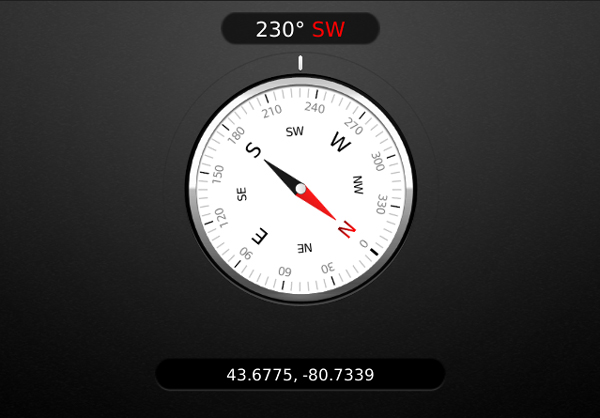
\includegraphics[scale=0.5]{MagnetometerApp.jpg}
\caption{a simple compass app that establishes the magnetometer sensor}
\end{figure}

\subsubsection*{Combined Sensors (6-axis approach)}
Combining accelerometer and gyroscope allows measurement of 6 orientations on X, Y and Z axis, allowing the apps to calculate placement of the device in the 3D environment more accurately.
\subsubsection*{9-axis approach}
Accelerometer, magnetometer, gyroscope could be all combined together for even more valuable user experience. For instance - enabling an online feature with more precise positioning in relation to other users could be considered. The data gathered from accelerometer, magnetometer and gyroscope can accurately position the artefact in the world, including the changes in position and rotation. On top of that, multiple sensors could fill individual sensors blind spots. 
%http://issuu.com/eeweb/docs/01-2015_embedded_developer_2_pages/30?e=7607911/11184384
%picture!!!

\begin{figure}[H]
\begin{subfigure}{.5\textwidth}
  \centering
  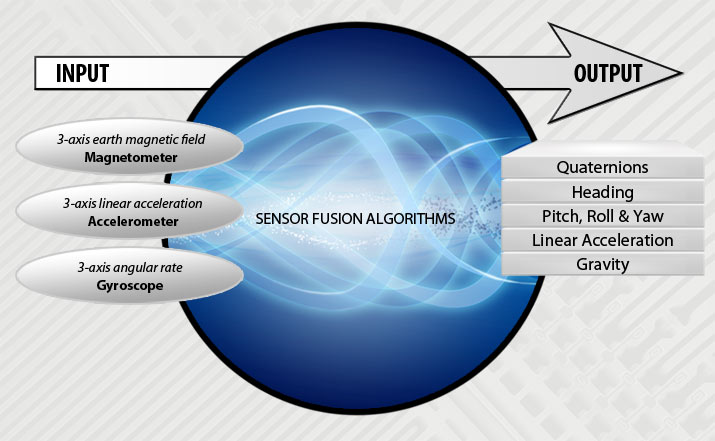
\includegraphics[width=.9\linewidth]{Sensors.jpg}
\end{subfigure}%
\begin{subfigure}{.5\textwidth}
  \centering
  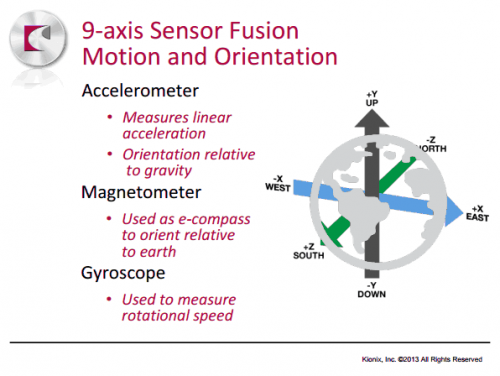
\includegraphics[width=.9\linewidth]{Sensors2.png}
\end{subfigure}
\caption{uses of sensors}
\end{figure}

\subsubsection*{Other sensors}
For example it is possible to create an app using microphone as the only input sensor, in one case the creators decided that the phone records sounds and plays it back in theme of The Batman Rises (http://darkknightrises.rjdj.me/).
\subsection{conclusion}
After gaining more knowledge it can be seen that there is a variety of options how to use sensors in apps. Whether it is all of them together or using only few of them, it is mandatory to take all the options into consideration. As the project theme mentions it, the project has to be with non-traditional user interface, meaning that this project should aim for more complex or more "interesting" choices regarding sensors or user input.
